\documentclass[12pt]{article}
\usepackage{titling}

\title{Adversarial Deep Neural Networks Effectively Remove Nonlinear Batch Effects from Gene-Expression Data}
\author{Jonathan B. Dayton}
% \author[1]{Jonathan B. Dayton}
% \author[1]{Stephen R. Piccolo}
% \affil[1]{Department of Biology, Brigham Young University, Provo, UT 84602 USA}
\date{2019}

% Times New Roman for the thesis submission
% \usepackage{mathptmx}
\usepackage{graphicx}
\usepackage{setspace}
\usepackage{authblk}
\usepackage{url}
\usepackage[inline,shortlabels]{enumitem}
\usepackage[square,numbers]{natbib}
% \usepackage{natbib}
\usepackage{floatrow}
\floatsetup[table]{capposition=top}
\usepackage[nomarkers,nolists,tabhead,fighead,tablesfirst]{endfloat}
% \renewcommand{\efloatseparator}{\mbox{}} % multiple figures per page
\usepackage[letterpaper,left=1in,right=1in,top=1in,bottom=1in]{geometry}
\usepackage{csvsimple}
\usepackage{multirow}
\usepackage[table]{xcolor}
\usepackage{changepage}
\usepackage{tocloft}
\usepackage[bookmarksnumbered,bookmarksopen=true,bookmarks=true]{hyperref}
\usepackage{bookmark}

% stuff for restyling the table of contents
\renewcommand\cftsecfont{\mdseries}
\renewcommand\cftsecpagefont{\mdseries}
\renewcommand{\contentsname}{\begin{center}\normalsize{\textnormal{TABLE OF CONTENTS}}\end{center}}
\renewcommand{\listtablename}{\begin{center}\normalsize{\textnormal{LIST OF TABLES}}\end{center}}
\renewcommand{\listfigurename}{\begin{center}\normalsize{\textnormal{LIST OF FIGURES}}\end{center}}

\bibliographystyle{unsrtnat}

\begin{document}

\pagenumbering{roman}
\begin{titlingpage}
	\setcounter{page}{1}
	\addcontentsline{toc}{section}{Title Page}
	\begin{center}
		\begin{adjustwidth}{+0.5in}{+0.5in}
			\begin{center}
				\doublespacing \thetitle\\ \singlespacing
			\end{center}
		\end{adjustwidth}
		\vfill
		\theauthor\\
		\vfill
		A thesis submitted to the faculty of\\
		Brigham Young University\\
		in partial fulfillment of the requirements for the degree of\\
		\vspace{1em}
		Master of Science\\
		\vfill
		Stephen R. Piccolo, Chair\\
		Mark Clement\\
		David Wingate\\
		\vfill
		Department of Biology\\
		\vspace{1em}
		Brigham Young University
		\vfill
		Copyright \textcopyright \ \thedate \ \theauthor\\
		\vspace{1em}
		All Rights Reserved
	\end{center}

\end{titlingpage}

% Title / abstract page
\begin{titlingpage}
	\setcounter{page}{2}
	\phantomsection
	\addcontentsline{toc}{section}{Abstract}
	\begin{center}
		ABSTRACT\\
		\vspace{1em}
		\begin{adjustwidth}{+0.5in}{+0.5in}
			\begin{center}
				\thetitle\\
			\end{center}
		\end{adjustwidth}
		\vspace{1em}
		\theauthor\\
		Department of Biology, BYU\\
		Master of Science
	\end{center}
	% \begin{abstract}
		Gene-expression profiling enables researchers to quantify transcription levels in cells, thus providing insight into functional mechanisms of diseases and other biological processes.
		However, because of the high dimensionality of these data and the sensitivity of measuring equipment, expression data often contains unwanted confounding effects that can skew analysis.
		For example, collecting data in multiple runs causes nontrivial differences in the data (known as batch effects),
		known covariates that are not of interest to the study may have strong effects,
		and there may be large systemic effects when integrating multiple expression datasets.
		Additionally, many of these confounding effects represent higher-order interactions that may not be removable using existing techniques that identify linear patterns.
		We created Confounded to remove these effects from expression data.
		Confounded is an adversarial variational autoencoder that removes confounding effects while minimizing the amount of change to the input data.
		We tested the model on artificially constructed data and commonly used gene expression datasets and compared against other common batch adjustment algorithms.
		We also applied the model to remove cancer-type-specific signal from a pan-cancer expression dataset.
		Our software is publicly available at \url{https://github.com/jdayton3/Confounded}.
	% \end{abstract}
	\vfill
	\noindent
	Keywords: batch effects, batch correction, gene expression, transcriptomics, deep learning, adversarial neural network, variational autoencoder
\end{titlingpage}

\doublespacing

\begin{titlingpage}
	\setcounter{page}{3}
	\phantomsection
	\addcontentsline{toc}{section}{Acknowledgments}
	\begin{center}
		ACKNOWLEDGMENTS\\
		TODO: Fill this out.
	\end{center}
\end{titlingpage}

\setcounter{page}{4}
\phantomsection
\addcontentsline{toc}{section}{Table of Contents}
\tableofcontents
\newpage
\phantomsection
\addcontentsline{toc}{section}{List of Tables}
\listoftables
\newpage
\phantomsection
\addcontentsline{toc}{section}{List of Figures}
\listoffigures
\newpage

% make bookmarks for Figure and Tables sections
\renewcommand{\figuresection}{\pdfbookmark[0]{Figures}{figure}Figures}
\renewcommand{\tablesection}{\pdfbookmark[0]{Tables}{table}Tables}

\pagenumbering{arabic}
\section{Background} \label{sec:background}

Gene expression data can be applied in many ways to advance our understanding of medicine and biology.
For example, expression data has been applied to discover conserved genetic modules \citep{stuart_gene-coexpression_2003}, to better understand the mechanisms of cardiovascular disease \citep{henriksen_application_2002}, to more accurately predict the clinical outcome in cancer patients \citep{veer_gene_2002}, and to discover effective drugs for treating specific diseases \citep{sirota_discovery_2011}.
Expression datasets are quite ``wide,'' often containing tens of thousands of columns representing each gene in the human transcriptome.
Because of the sensitive nature of these data (i.e. gene product levels in organisms may respond drastically to small environmental changes) and of the equipment used to quantify expression levels, expression data often contains unwanted confounding effects that can skew analysis.
Three examples of this include
\begin{enumerate*}[(a)]
	\item batch effects, \label{it:batch}
	\item known covariates, and \label{it:cov}
	\item dataset-level effects. \label{it:int}
\end{enumerate*}
\ref{it:batch} Batch effects occur when expression data are generated in multiple runs or multiple batches, and slight systemic differences occur during the different runs, such as different technicians operating the machine or slight temperature differences in the room.
Batch effects are understood to have a nontrivial impact on high-throughput expression data \citep{leek_tackling_2010}.
In one study, researchers found that, contrary to previous knowledge, expression values from mice and humans clustered more closely by species than by tissue type \citep{yue_comparative_2014};
however, referees showed in a rebuttal that when accounting for batch effects, these data actually clustered more closely by tissue type, as initially expected \citep{gilad_reanalysis_2015}.
\ref{it:cov} Systemic bias can be even more pronounced when there are known covariates---for example, using data collected from different cancer types when cancer type is not of interest to the study \citep{dayton_classifying_2017-1}.
\ref{it:int} Finally, though batch effects within a dataset collected all by one lab at one time may be somewhat decreased experimentally by careful replication of experimental conditions, this is no longer possible when integrating different datasets;
however, much better statistical significance can be achieved when analyzing larger datasets, so data integration is a key goal for transcriptomic analysis  \citep{lazar_batch_2013}.
Each of these problems---batch effects, known covariates, and dataset integration---represents a case where data measurements are effected by some hidden variables and must be removed for effective analysis (see Figure \ref{fig:workflow}).


\begin{figure}
	\pdfbookmark[1]{Figure \ref{fig:workflow}}{workflow}
	\centering
	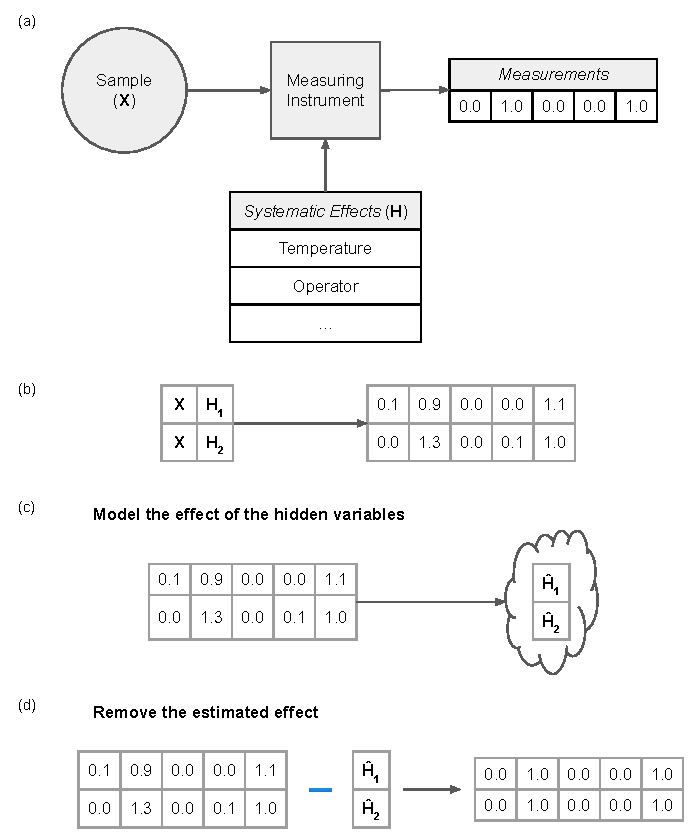
\includegraphics[width=\columnwidth]{figures/final/adjuster_workflow.pdf}
	\caption[Batch adjustment justification and steps]{\textbf{Batch adjustment justification and steps.}
	\begin{enumerate*}[(a)]
		\item When measurements are collected from a sample ($X$), systemic effects ($H$) also affect the measurements.
		\item If data from the same sample $X$ is measured under two different conditions, $H_1$ and $H_2$, we may obtain slightly different measurements.
		\item In order to normalize batches of data relative to one another, we first estimate the effect of the hidden variables based on differences in measurements between batches.
		\item Second, we remove the estimated effects in order to normalize the batches relative to one another.
	\end{enumerate*}
	}
	\label{fig:workflow}
\end{figure}

Several methods exist for removing batch effects from gene expression datasets.
Two commonly used methods are ComBat \citep{johnson_adjusting_2007} and SVA \citep{leek_capturing_2007}.
ComBat uses an empirical Bayes method to estimate batch effect parameters and then uses linear regression to remove the effects, and SVA uses singular value decomposition to model batch effects which can then be accounted for in statistical analyses.
Since both of these methods use linear methods to model confounding effects, they are not designed to account for nonlinear effects, such as the cascading changes in gene pathways in response to environmental stressors (e.g. gene X transcripts increase and gene Y transcripts decrease in response to rising temperature, and since both are now past a certain threshold, gene Z transcripts also increase, and so on).
As machine learning becomes more common in biological research, these nonlinear confounding effects become more troublesome since many machine learning algorithms can successfully identify complex interactions between variables.
For example, advances in neural networks have introduced new ways to account for higher-order, nonlinear relationships in data.
These networks have proven effective in removing irrelevant, domain-specific signal in credit rating, online reviews, and image recognition tasks \citep{louizos_variational_2015}.
Recent work \cite{shaham_removal_2017,shaham_batch_2018,upadhyay_removal_2019} has applied neural networks to batch effects.
However, several limitations complicate their usability on many real-world datasets:
they require that the input data only contains two batches, that the batches are sufficiently large (we received errors when testing with a subset of MNIST where n=100), and that the batches are perfectly balanced.
These requirements rarely hold in existing datasets; for example, the bladderbatch dataset used in the R sva package \cite{leek_bladderbatch_2017,leek_sva_2017} has 5 batches, only 57 samples, and between 4 and 19 samples per batch.
Additionally, the metrics these studies have used to validate results don't test whether complex interactions still remain in the data.

To address these issues, we implemented a deep neural network approach to batch correction that works on real-world datasets, and we calculated batch removal measurements based on machine learning algorithms to test for remaining nonlinear effects.
Artificial neural networks are a machine learning tool inspired by the way human brains function; input values pass through layers of linear and nonlinear functions, the final output values are measured against objectives, and the layers of functions are adjusted to bring the outputs closer to the objectives.
This process is repeated until the outputs are sufficiently close to their targets \citep{schmidhuber_deep_2015}.
Research has shown that neural networks are effective in working with gene expression data; for example, neural networks have been applied
to detect cancer and identify critical cancer genes \citep{danaee_deep_2016},
to infer gene-expression values from just the values of a few ``landmark genes'' \citep{chen_gene_2016},
to extract biologically relevant latent spaces in RNA-Seq data \citep{way_extracting_2017},
to reduce the dimensions of single-cell RNA-Seq data \citep{lin_using_2017},
to identify drug-repurposing targets using transcriptomic data \citep{aliper_deep_2016},
and to generate realistic synthetic biomedical data for other scientific studies \citep{beaulieu-jones_privacy-preserving_2017}.
Autoencoders are a type of neural network that encode and then reconstruct their input, and their traditional objective function is to construct the output to be as similar to the input as possible \citep{hinton_reducing_2006}.
Neural networks have historically decreased in effectiveness when working with data from multiple research domains \citep{ganin_domain-adversarial_2015}, in part because they may learn based on dataset-specific confounding effects (e.g. which researcher collected the data) instead of learning based on practically meaningful causal effects (e.g. which gene is consistently upregulated in a disease) \citep{louizos_causal_2017-2}.
Recently, researchers have experimented with discouraging neural networks from learning based on domain-specific information by giving them two objective functions:
1. to learn as much as possible about the input data and
2. to forget any patterns that help distinguish between domains \citep{ganin_domain-adversarial_2015,tzeng_deep_2014-2}.
\citet{louizos_variational_2015} used this type of dual objective function with a variational autoencoder and successfully removed domain-based variability in credit score, financial savings, and hospital admittance datasets.

In this study, we present Confounded, an adversarial autoencoder that identifies and removes confounding effects.
We test the hypothesis that using an adversarial neural network can correct for confounding effects more completely than previous tools do.
We also explore the extent to which confounders still remain in different datasets after adjustment with various algorithms, and we present a framework to assess the extent to which confounding effects remain after adjustment using various classification algorithms.

\section{Methods} \label{sec:methods}

All our code has been made publicly available at \url{https://github.com/jdayton3/Confounded}, and all our data are available as described below.

\subsection{Network Structure}

We used an adversarial autoencoder network to model and remove the confounding effects.
We structured this network in two parts: a variational autoencoder \cite{louizos_variational_2015} to replicate the input (expression) data and a discriminator to detect remaining confounding effects in the autoencoder's output.
By penalizing the autoencoder for the discriminator's success, the autoencoder subnetwork learned over the course of training to output the expression data with confounding effects minimized.
We implemented the neural network in TensorFlow 1.11.0 \cite{abadi_tensorflow_2015} with Python 3.6 \cite{python_software_foundation_python_2019}.
All layers in the network were fully connected and all activation functions were Rectified Linear Units (ReLUs) \cite{agarap_deep_2018} except the final layers in the autoencoder and the discriminator, which used the sigmoid function.

\begin{figure}
	\pdfbookmark[1]{Figure \ref{fig:network}}{network}
	\centering
	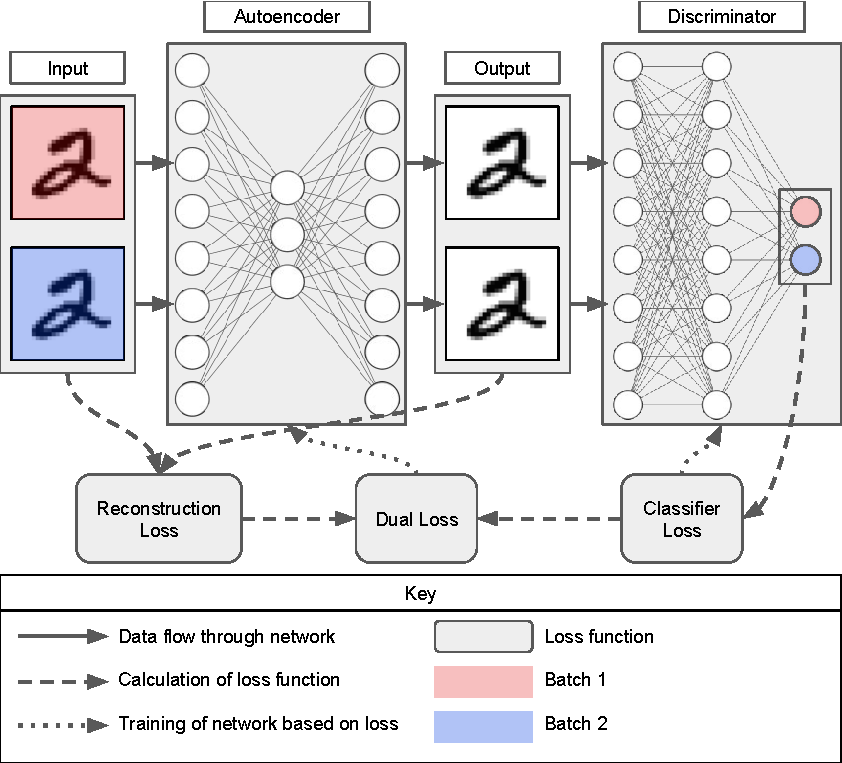
\includegraphics[width=\columnwidth]{figures/final/network.pdf}
	\caption[Network architecture of Confounded]{\textbf{Network architecture} of Confounded.
	Data with batch effects (represented by different colors) are input into an autoencoder.
	The output of the autoencoder is classified by a discriminator network based on batch.
	The autoencoder is then penalized based on the success of the discriminator.
	Over time, the autoencoder learns to output a faithful representation of the data without signal due to batch.}
	\label{fig:network}
\end{figure}

\subsubsection{Autoencoder}

We implemented the variational autoencoder \citep{louizos_variational_2015} described by \citet[Chapter 15]{geron_hands-machine_2017}.
This network has 2 hidden encoding layers and 2 decoding layers, each of size 500.
The code size is 20.
Each hidden layer is activated with the Exponential Linear Unit (ELU) function \citep{clevert_fast_2015}.
It is trained with the Adam optimizer \citep{kingma_adam_2014} on reconstruction loss (sigmoid cross entropy) combined with latent loss (KL divergence \citep{kullback_information_1951}).

\subsubsection{Discriminator}

We trained the discriminator to determine the original batch of the autoencoder's output.
The discriminator subnetwork consists of an input layer; four fully connected hidden layers of sizes 1024, 512, 512, and 128, respectively; and an output layer sized based on the number of batches.
In order to combat overfitting and improve training, we also added 50\%-probability dropout \cite{srivastava_dropout_2014} (which prevents overfitting by dropping a random subset of layer inputs in each training iteration) and batch normalization \cite{ioffe_batch_2015} (which helps training by smoothing out the optimization landscape \citep{santurkar_how_2018}) to each layer of the discriminator.
These additions seemed to reduce overfitting in the discriminator.

\subsubsection{Loss functions}

We trained the network using three loss functions.
First, we calculated the autoencoder's loss ($L_A$) by summing the reconstruction loss (sigmoid cross entropy between the autoencoder's input and output) and the latent loss (Kullback-Leibler (KL) divergence \cite{kullback_information_1951} of the code layer).
Second, we calculated the discriminator's loss ($L_D$) as sigmoid cross entropy between its output and a one-hot encoding of the samples' batch labels.
Finally, we also trained the autoencoder layers on a combination of the two previous losses,

\begin{equation}
	\label{dual_loss}
	L_{dual} = L_A - \lambda{}(L_D)
\end{equation}

The $\lambda$ value represents a tradeoff parameter for tuning the network's tendency for more faithfully replicating the input or for more completely removing confounding effects.
A higher $\lambda$ value indicates that the network should remove confounding effects more aggressively, whereas a lower value indicates that the network should instead favor faithfully reconstructing the input data.
We did not optimize $L_A$ directly; instead we trained the autoencoder by optimizing $L_{dual}$.

\subsubsection{Training}

In all cases, we trained the network using the Adam Optimizer \citep{kingma_adam_2014} with a training rate of 0.0001 for 10,000 iterations on mini-batches of size 100.
In each iteration, we optimized on both $L_D$ and $L_{dual}$.
When optimizing $L_D$ (i.e. training the discriminator), we froze the autoencoder's weights, and vice versa.
We trained the network on a 2017 Dell XPS 15 9560 with an 8-core Intel i7-7700HQ CPU and 16 GB of RAM.
For each dataset, training typically took roughly 30 minutes to complete, including the time taken to load the input into memory and to save the output to disk.

\begin{figure}
	\pdfbookmark[1]{Figure \ref{fig:training_loss}}{training_loss}
	\centering
	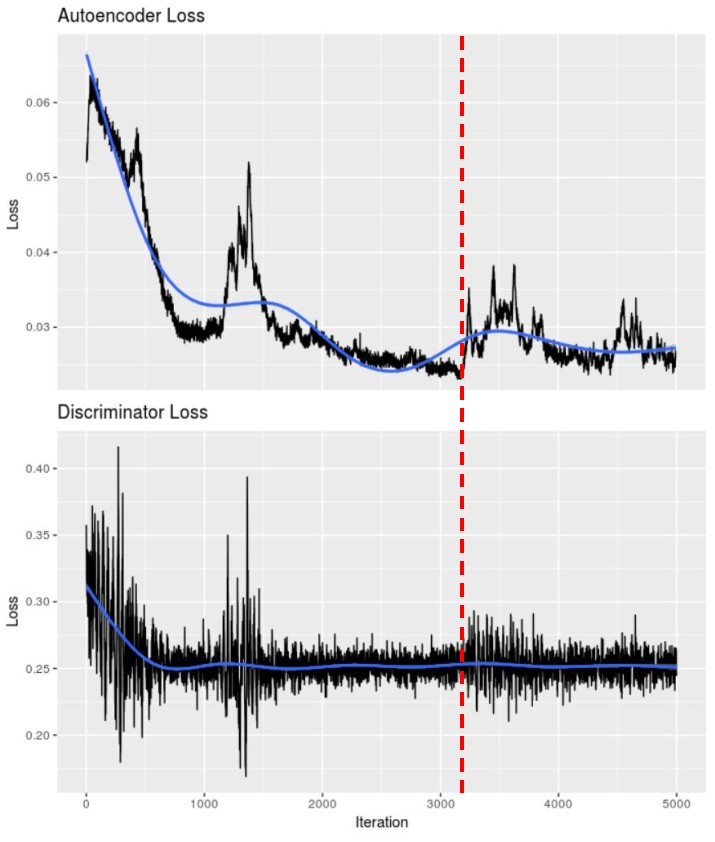
\includegraphics[width=\columnwidth]{figures/final/training_loss.pdf}
	\caption[Autoencoder and discriminator loss]{\textbf{Autoencoder and discriminator loss} over time for one run of Confounded on the MNIST dataset.
	Over the course of training, the autoencoder more faithfully replicates the input data.
	The autoencoder also seems to introduce noise (see the red dashed line around iteration 3100) in response to the discriminator's slight improvements.}
	\label{fig:training_loss}
\end{figure}

\subsection{Datasets}

In order to test both theoretical and practical differences between Confounded and previous methods, we compared them for a variety of datasets of varying sizes and type of data measured.

\begin{table}
	\centering
	\begin{tabular}{|p{0.18\linewidth}|p{0.14\linewidth}|p{0.1\linewidth}|p{0.15\linewidth}|p{0.23\linewidth}|p{0.16\linewidth}|}
  \hline
  Dataset         & Dimensions   & Number of Batches & Batch Label      & True Class Label       & Data Type        \\
  \hline
  Bladder Batch   & $57\times22,283$  & 5                 & Batch            & Cancer status          & Microarray       \\
  \hline
  GSE37199        & $93\times20,024$  & 2                 & Plate            & Cancer stage           & Microarray       \\
  \hline
  MNIST           & $10,000\times784$ & 2                 & Artificial batch & Digit                  & Grayscale images \\
  \hline
  TCGA Pan-Cancer & $9,366\times325$  & 25                & Cancer Type      & TP53 mutation presence & RNA-Seq \\
  \hline
\end{tabular}

	\caption[Dataset information]{
		\pdfbookmark[1]{Table \ref{tab:datasets}}{datasets}
		\textbf{Dataset information} for each dataset used.
	}
	\label{tab:datasets}
\end{table}

\subsubsection{MNIST}

The MNIST digits dataset \cite{lecun_mnist_nodate} is a database of images of handwritten digits that are size-normalized and centered.
It contains 60,000 training images and 10,000 test images.
We used MNIST so we could visually assess how well the true signal (in this case, the shape and digit of each handwritten digit image) was preserved after batch adjustment.
In order to use this dataset, we flattened each 28 by 28 image into a 1D vector of size 784 and put each in a CSV file along with the accompanying digit information.
We limited our dataset to only the 10,000 test images.
Although convolutional layers are typically used when working with image data, we only used fully connected layers even for this image dataset.
In this way, we show that the autoencoder is still able to find and represent spatial relationships without explicitly defining spatial relationships in the model while testing the same network we use on expression data, where no spatial relationships are inherent.

\paragraph{Synthetic Batch Effects}

Because there is no batch information in the MNIST digits dataset, we had to simulate nonlinear confonding effects.
To do so, we wrote a Python script to take the MNIST data in, apply a nonlinear effect, and output the adjusted data.
We applied nonlinear effects by iteratively realizing vectors of normally distributed values, multiplying and adding these vectors to the ``expression'' vectors, and applying nonlinearity to the adjusted vector.
We split the image data into two batches while keeping the batches balanced (5,000 images for each batch) and including the same number of each digit in each batch.
We applied the same random vectors to each image in a batch.
Finally, we added random noise to each image in order to prevent images in a batch from being overly similar to each other.

\subsubsection{Bladderbatch}

The bladderbatch dataset is a microarray transcriptomic expression dataset from a study of patients with bladder cancer \cite{dyrskjot_gene_2004}.
It has been made available as an R package \cite{leek_bladderbatch_2017} and is used in the documentation of the sva R package \cite{leek_sva_2017} to illustrate how to batch-adjust using ComBat.
It contains expression values for 57 tissue samples with and without bladder cancer across 5 unbalanced batches.
The dataset has a cancer status (cancerous vs. normal tissue) column, which we used for ``true class'' classification, and a batch column.
Because bladderbatch is such a small dataset in terms of typical deep learning datasets, we selected it as a way to test whether our network was overfitting.

\subsubsection{GSE37199}

The GSE37199 dataset contains Affymetrix microarray gene-expression data from patients with advanced castration-resistant prostate cancer \cite{olmos_prognostic_2012}.
We accessed a version of this dataset from \url{http://doi.org/10.17605/OSF.IO/SSK3T} that was tidied as part of a curated compendium of human transcriptional biomarker data \cite{golightly_curated_2018}.
It contains expression values for 93 tissue samples categorized as either ``Advanced castration resistant'' or ``good prognosis.''
We used this cancer status variable as the ``true class'' for classification.
It has two types of batch variables: ``plate'' and ``centre.''
We adjusted against the ``plate'' variable because it was more balanced than ``centre'' (with counts of $\{43, 50\}$ compared to $\{27, 66\}$).
The GSE37199 dataset represents a slightly larger dataset than bladderbatch, with only two batches that are closer to being balanced (with batch counts of $\{4, 5, 11, 18, 19\}$ and $\{43, 50\}$, respectively).

\subsubsection{TCGA Pan-cancer Data}

The Cancer Genome Atlas (TCGA) Pan-Cancer project produced expression data for thousands of tumors across many cancer types \cite{the_cancer_genome_atlas_research_network_cancer_2013}.
In a previous study \cite{dayton_classifying_2017-1}, we classified this dataset based on the presence or absence of mutations in several known cancer genes.
We attempted to adjust for the confounding effect of cancer type using ComBat prior to classification.
However, we found that a strong nonlinear signal could still be identified by the Random Forests algorithm after adjustment.
Here, we used the same version of the dataset that we tidied in this previous study (available at \url{https://osf.io/7xjdn/}).
This dataset has RNA-Seq expression values for 9,365 samples across 25 distinct cancer types.
We used this dataset as a way to test whether Confounded works on RNA-Seq data and to test whether we could remove confounding effects that ComBat cannot remove.

\subsection{Comparison to other methods}

We compared our method to two other batch adjusters: a scale adjuster and ComBat \citep{johnson_adjusting_2007}.
We implemented the scale adjuster in the R programming language, version 3.6.0 \citep{r_core_team_r_2014} using RStudio version 1.2.1194 \citep{rstudio_team_rstudio_2018}.
It adjusts the data by linearly expanding or contracting each batch so all batches have the same range.
We used the ComBat implementation from the R sva package \citep{leek_sva_2017} with some modifications to allow it to work on columns without variance in the MNIST dataset.
We initially intended to test against the SVA \citep{leek_capturing_2007} method but concluded that SVA is more suited for producing surrogate variables for further statistical research rather than removing those variables from the data.
There are a number of other methods for batch adjustment that do and do not use deep neural networks (for example, see \citep{leek_capturing_2007,espin-perez_comparison_2018,shaham_removal_2017,shaham_batch_2018}). % TODO: add like 8 more methods
Unfortunately, most of these methods lack a common interface and common assumptions that input datasets must meet.
For these reasons, we compared Confounded only to the two methods listed above.
Future batch adjustment research may benefit from standardization of input formats, user interfaces, and validation datasets.

\subsection{Statistics and Metrics}

\subsubsection{Mean squared error}

Mean squared error (MSE) is a measure of how much two vectors or matrices deviate from one another.
It is commonly used as a loss value in autoencoders to make the network minimize the difference between the input and output values.
We wanted to see how well Confounded and other batch correction software maintain patterns in the input data as measured by MSE.

\subsubsection{Maximum mean discrepancy} \label{section:mmd}

In a recent paper, \citet{shaham_removal_2017} used neural networks to remove batch effects.
Instead of constraining the autoencoder to remove batch effects based on a discriminator, these researchers trained their network to minimize maximum mean discrepancy (MMD) between batches in an embedded layer of their network.
We calculated MMD using the same formula as \citeauthor{shaham_removal_2017} to determine whether batches looked like they came from the same distribution after adjustment.
For the kernel, we used the Gaussian kernel between two batches as implemented in \texttt{sklearn.metrics.pairwise.rbf\_kernel} \cite{pedregosa_scikit-learn_2011}.
In cases where there were more than two batches, we averaged all pairwise MMD values to calculate an overall MMD.

\subsubsection{Classification accuracy}

In order to determine \begin{enumerate*}[(a)]
	\item whether batch can still be identified post-adjustment and
	\item how well class-related signal is maintained after adjustment,
\end{enumerate*}
we determined classification accuracy based on batch and ``true class'' labels using several machine learning classifiers.

We used four classifiers from the scikit-learn 0.19.1 Python library \cite{pedregosa_scikit-learn_2011} in order to classify on batch and true class before and after adjustment: Naive Bayes \citep{maron_automatic_1961}, Random Forests \citep{tin_kam_ho_random_1995}, k-Nearest Neighbors \citep{fix_discriminatory_1951}, and SVM \citep{cortes_support-vector_1995} with a radial basis kernel.
Table \ref{tab:datasets} details which columns were used for training.

We calculated the average of classification accuracies for four-fold cross-validation repeated three times.
We interpret lower accuracy for batch classification as meaning that the batch is removed more effectively.
We also interpret higher true class classification as meaning that the important signal is not lost during the process of adjustment.
Therefore, given output data from the ideal batch adjuster, batch classification would be no better than random for any classification algorithm, and true class accuracy would be no lower than accuracy for the unadjusted data.

\section{Results} \label{sec:results}

The scaling method performed consistently worse across the qualitative and quantitative evaluations that we performed;
ComBat and Confounded performed relatively well overall, but each of these algorithms excelled in different types of scenarios, which we illustrate below.

\subsection{Confounded removes nonlinear confounding effects that other adjusters miss}

Various previous studies use differing methods to show qualitatively and quantitatively how well confounding effects have been removed.
To compare Confounded to other batch adjustment methods, we compared PCA and t-SNE plots along with MSE, MMD, and classifier batch prediction accuracy (using various classifiers).

PCA and t-SNE plots seem to show a decrease in separability after adjustment with various methods for the GSE37199 dataset (see Figures \ref{fig:pca} and \ref{fig:tsne}).
However, previous research has shown that these plots are not completely trustworthy in representing nonlinear effects \cite{dayton_classifying_2017-1}.
In the PCA plot, Confounded appears to maintain a similar distribution to the unadjusted data, indicating that the underlying distribution has been faithfully reproduced by the networks.
The t-SNE plot shows that the data post-adjustment by Confounded and ComBat appear to cluster less tightly by batch than the unadjusted and scale-adjusted data.
This may indicate an effective removal of nonlinear effects in both cases.

\begin{figure}
	\pdfbookmark[1]{Figure \ref{fig:pca}}{pca}
	\centering
	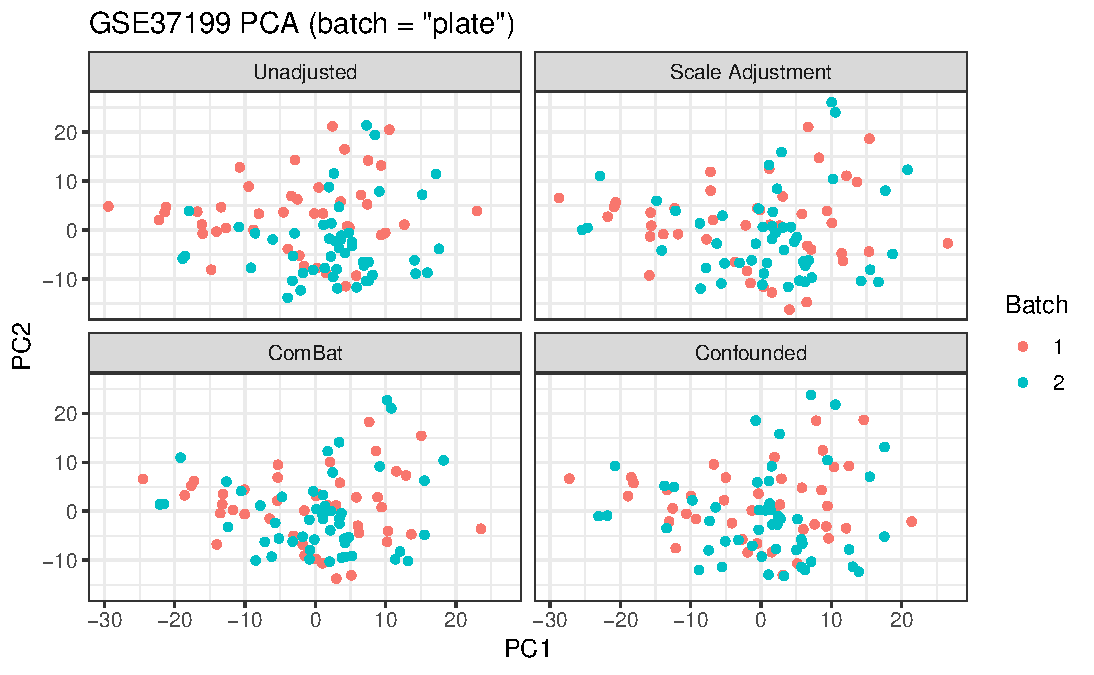
\includegraphics[width=\columnwidth]{figures/final/pca.pdf}
	\caption[Principal components analysis (PCA)]{\textbf{Principal components analysis} (PCA) of the GSE37199 dataset before and after batch adjustment with various adjusters.
	None of the datasets appear to be linearly separable.
	Confounded appears to maintain the same distribution of data overall as the unadjusted data while perhaps aligning the batches' distributions.}
	\label{fig:pca}
\end{figure}
\begin{figure}
	\pdfbookmark[1]{Figure \ref{fig:tsne}}{tsne}
	\centering
	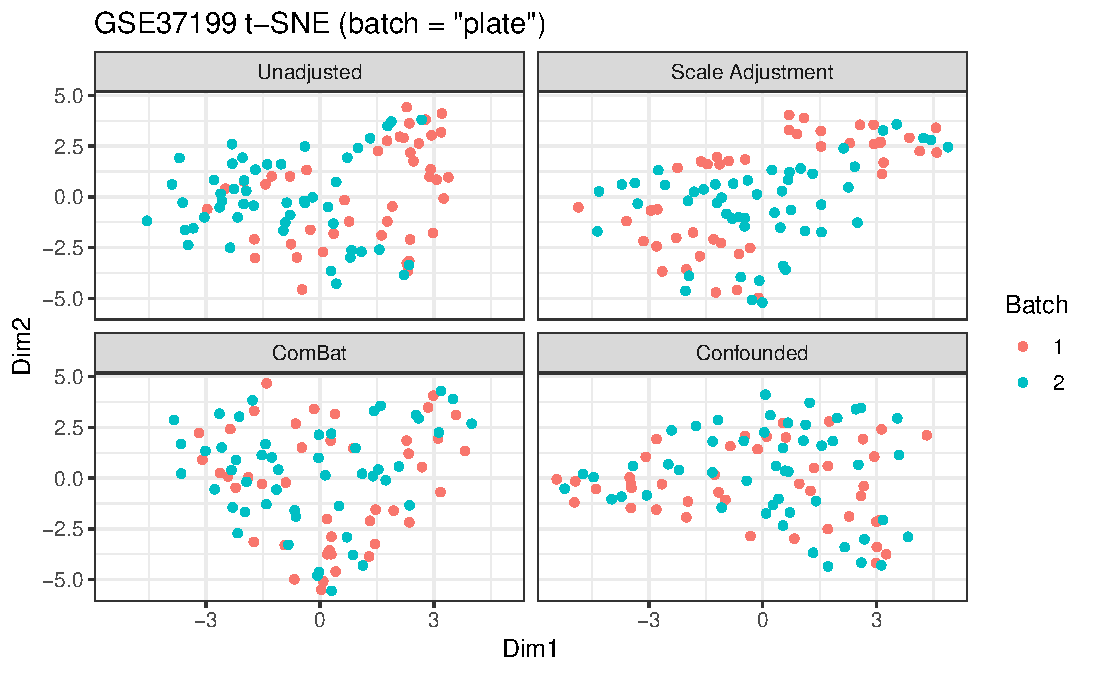
\includegraphics[width=\columnwidth]{figures/final/tsne.pdf}
	\caption[T-distributed Stochastic Neighbor Embedding (t-SNE)]{\textbf{T-distributed Stochastic Neighbor Embedding} (t-SNE) plot for the GSE37199 dataset before and after adjustment with several algorithms.
	The data seem to cluster less by batch for both Confounded and ComBat, indicating that both adjusters may be removing nonlinear effects in this dataset.}
	\label{fig:tsne}
\end{figure}

Confounded shows mixed success with the MSE and MMD metrics.
With MSE, Confounded outperformed the scale adjuster in 3 of the 4 datasets but scored drastically worse on the MNIST dataset, with scores (listed as: scale, Confounded) of \{(0.003, 0.00168), (0.247, 0.0698), (0.00312, 0.0187), (912315, 139458)\}.
With MMD, Confounded outperformed the scale adjuster again in 3 of the 4 datasets and tied the scale adjuster on the TCGA dataset, with scores of \{(0.463, 0.258),(0.0906, 0.0376),(0.0653, 0.0117),(0.0942, 0.0942)\}.
With both metrics, Confounded consistently performed somewhat worse than ComBat.
(See Figures \ref{fig:mse} and \ref{fig:mmd}.)

\begin{figure}
	\pdfbookmark[1]{Figure \ref{fig:mse}}{mse}
	\centering
	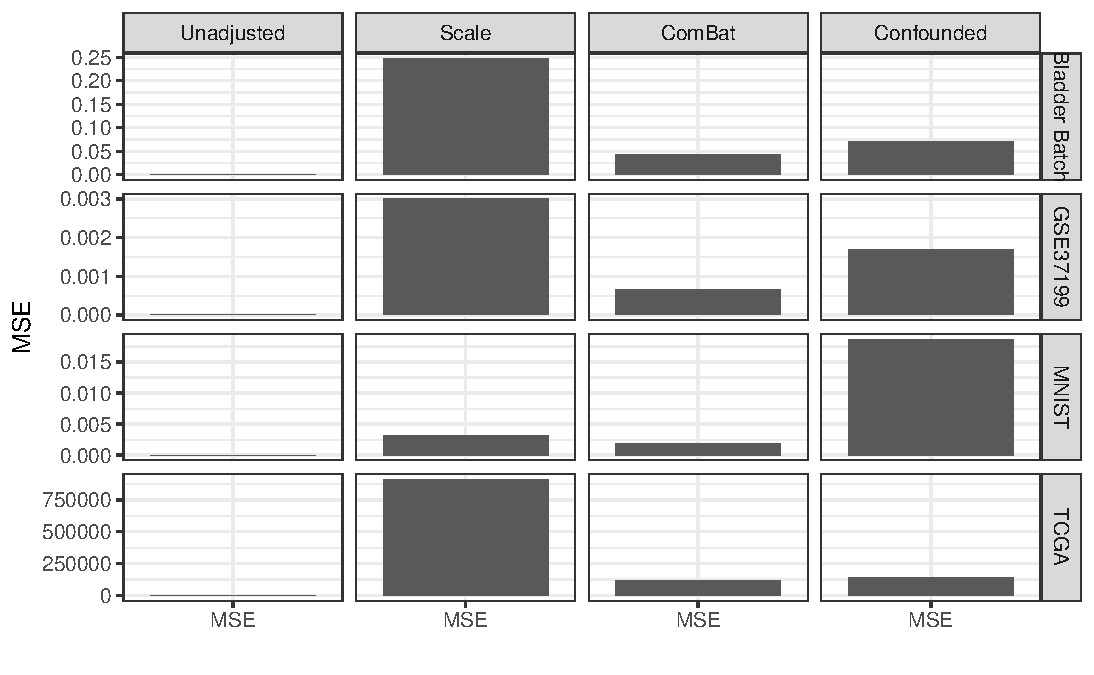
\includegraphics[width=\columnwidth]{figures/final/mse.pdf}
	\caption[Mean squared error (MSE)]{\textbf{Mean squared error} (MSE) between the data prior to and after adjustment with various algorithms.
	Lower MSE represents that the adjuster has more faithfully reproduced the input data.
	MSE for unadjusted data will always be 0 because the input data is identical to the output data.
	Confounded usually performs better than the scale adjuster and somewhat worse than ComBat when measuring MSE.}
	\label{fig:mse}
\end{figure}
\begin{figure}
	\pdfbookmark[1]{Figure \ref{fig:mmd}}{mmd}
	\centering
	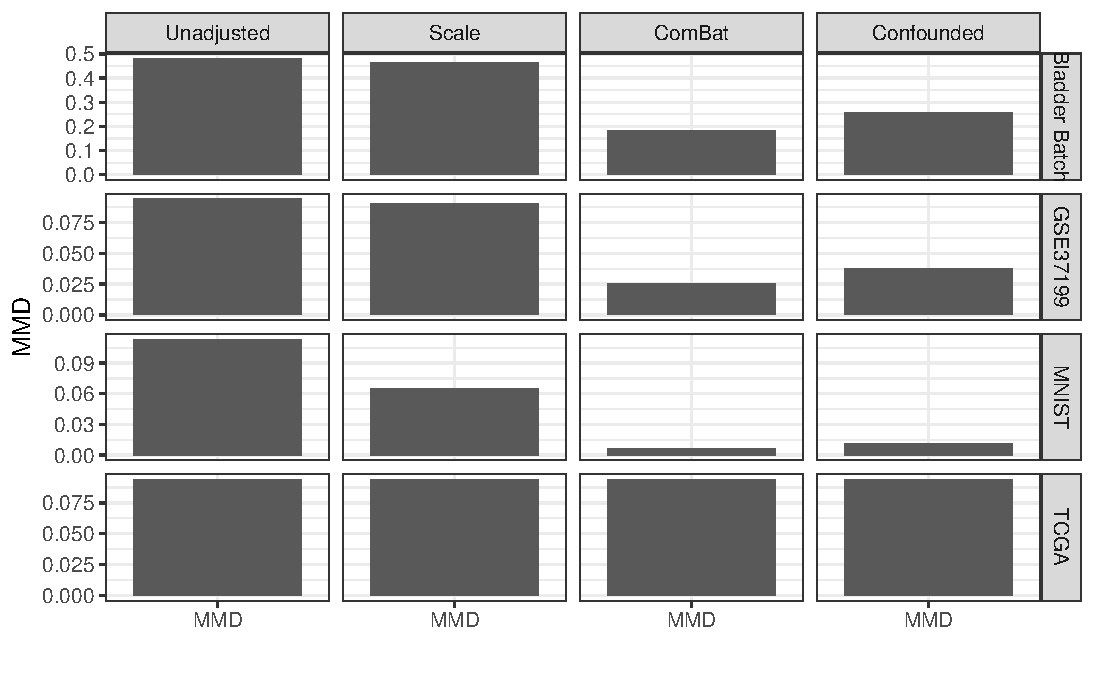
\includegraphics[width=\columnwidth]{figures/final/mmd.pdf}
	\caption[Maximum mean discrepancy (MMD)]{\textbf{Maximum mean discrepancy} (MMD) between different batches. Lower MMD indicates that the distributions of the different batches are more similar.
	In cases with more than two batches, MMD is computed pairwise between each batch and averaged.
	In each case, Confounded usually performs better than the scale adjuster and somewhat worse than ComBat when measuring MSE.}
	\label{fig:mmd}
\end{figure}

We would expect that after batch adjustment by an ideal adjuster, batch would no longer be detectable by any machine learning classifier.
Using the batch classification accuracy metric, Confounded seems to outperform other adjusters on larger datasets, whereas ComBat and Confounded seem to perform about the same on smaller datasets (see Figure \ref{fig:batch}).
With both the bladderbatch and GSE37199 datasets, batch classification accuracy decreases well below baseline after batch adjustment with ComBat for all classifiers we tested (see Table \ref{tab:batch}).
Interestingly, batch accuracy also decreases drastically for the MNIST and TCGA datasets, but only for the Naive Bayes classifier.
This may be due to two factors: both ComBat and Naive Bayes use Bayesian methods, so ComBat may specifically remove the effects that Naive Bayes identifies; and Naive Bayes does not find patterns based on interactions between variables.
Although Naive Bayes is no longer able to identify confounding effects in the data after ComBat-adjustment, Random Forests (which does use interactions between variables) still has a very high accuracy for MNIST and an increased accuracy for TCGA.
In contrast, after adjustment by Confounded, the Random Forests algorithm's accuracy decreases more than with any other adjuster for both the MNIST and TCGA datasets.
This indicates that while ComBat's performance may work at least as well as Confounded for smaller expression datasets, Confounded may work better with larger datasets.

\begin{figure}
	\pdfbookmark[1]{Figure \ref{fig:batch}}{batch}
	\centering
	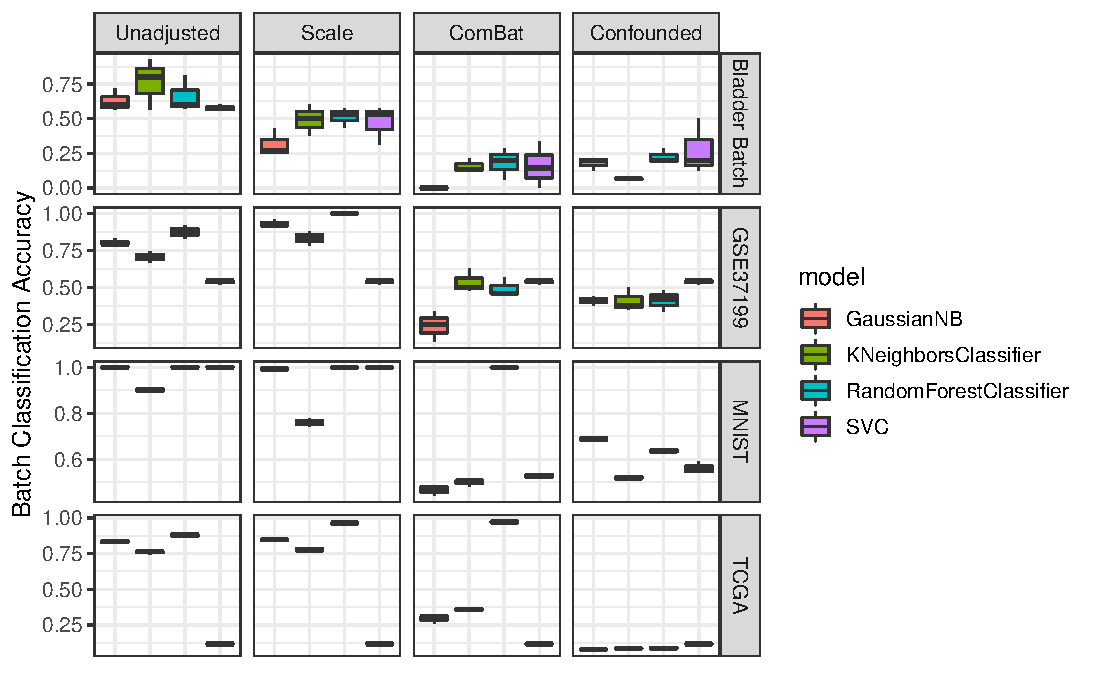
\includegraphics[width=\columnwidth]{figures/final/batch_accuracy.pdf}
	\caption[Batch classification accuracy]{\textbf{Batch classification accuracy} from 4-fold cross-validation repeated 3 times for several classifiers.
	Lower batch accuracy indicates that more batch-related signal has been removed and therefore indicates better performance.
	Confounded's performance is similar to ComBat's for the smaller datasets and is improved for the larger datasets.
	See also Table \ref{tab:batch}.}
	\label{fig:batch}
\end{figure}
\begin{table}
	\centering
	\centering
\begin{tabular}{l|l|r|r|r}
\hline
Dataset & Adjustment & Baseline & GaussianNB & RandomForest\\
\hline
\rowcolor{gray!6}   & unadjusted &  & 0.626 & 0.688\\
\cline{2-2}
\cline{4-5}
 & scale &  & 0.315 & 0.450\\
\cline{2-2}
\cline{4-5}
\rowcolor{gray!6}   & combat &  & 0.000 & 0.114\\
\cline{2-2}
\cline{4-5}
\multirow[t]{-4}{*}{\raggedright\arraybackslash bladderbatch} & confounded & \multirow[t]{-4}{*}{\raggedleft\arraybackslash 0.333} & 0.386 & 0.315\\
\cline{1-5}
\rowcolor{gray!6}   & unadjusted &  & 0.803 & 0.832\\
\cline{2-2}
\cline{4-5}
 & scale &  & 0.930 & 0.928\\
\cline{2-2}
\cline{4-5}
\rowcolor{gray!6}   & combat &  & 0.238 & 0.423\\
\cline{2-2}
\cline{4-5}
 & confounded &  & 0.338 & 0.353\\
\cline{2-2}
\cline{4-5}
\rowcolor{gray!6}  \multirow[t]{-5}{*}{\raggedright\arraybackslash gse37199} & NA & \multirow[t]{-5}{*}{\raggedleft\arraybackslash 0.538} & 0.662 & 0.670\\
\cline{1-5}
 & unadjusted &  & 0.996 & 1.000\\
\cline{2-2}
\cline{4-5}
\rowcolor{gray!6}   & scale &  & 0.998 & 1.000\\
\cline{2-2}
\cline{4-5}
\multirow[t]{-3}{*}{\raggedright\arraybackslash noisy} & combat & \multirow[t]{-3}{*}{\raggedleft\arraybackslash 0.500} & 0.698 & 1.000\\
\cline{1-5}
\rowcolor{gray!6}   & unadjusted &  & 0.832 & 0.879\\
\cline{2-2}
\cline{4-5}
 & scale &  & 0.846 & 0.965\\
\cline{2-2}
\cline{4-5}
\rowcolor{gray!6}  \multirow[t]{-3}{*}{\raggedright\arraybackslash tcga} & combat & \multirow[t]{-3}{*}{\raggedleft\arraybackslash 0.117} & 0.293 & 0.960\\
\hline
\end{tabular}
	\caption[Batch classification accuracy]{
		\pdfbookmark[1]{Table \ref{tab:batch}}{batch}
		\textbf{Batch classification accuracy} for several datasets and adjusters.
		The ideal batch adjuster would completely remove all signal due to batch and would therefore \textit{decrease} batch classification accuracy to around the baseline for all classifiers.
		See also Figure \ref{fig:batch}.
	}
	\label{tab:batch}
\end{table}

With the larger datasets in particular, Confounded outperforms the other adjusters.
On the MNIST dataset, Random Forests is able to detect batch with perfect or near-perfect accuracy after adjustment with the scale adjuster and ComBat, but the highest batch classification accuracy after adjustment by Confounded is Naive Bayes, with an accuracy of 68.8\%.
With TCGA, both the scale adjuster and ComBat drastically increase Random Forests' batch classification accuracy from 87.6\% to 96.3\% and 97.1\% respectively, whereas Confounded decreases the accuracy to 8.8\%.

\subsection{Class-related signal is still detectable after adjustment by Confounded}

With the smaller datasets, Confounded seems to keep true class information roughly as well as ComBat, (with Random Forests, Bladderbatch: 74.3 for ComBat\% and 72.1\% for Confounded, GSE37199: 60.4\% for ComBat and 69.0\% for Confounded; see Figure \ref{fig:true_class} and Table \ref{tab:true_class}).
For the Bladderbatch dataset, true class accuracy is much lower after adjusting with any algorithm, indicating that cancer status and batch may not be independent.

With the larger datasets, Confounded's true class accuracy consistently decreases below the accuracy of other adjusters.
A look at the MNIST digits before and after adjustment (see Figure \ref{fig:mnist}) shows that Confounded's output is often blurry, as is common with the output of variational autoencoders \cite{hou_deep_2016}.
With MNIST, Confounded's accuracy with Random Forests is still much higher than baseline (84.8\% vs. 11.4\%), but with TCGA, the accuracy decreases below baseline (66.5\% vs. 69.8\%) while the other adjusters' accuracies remain above baseline.
However, the particular set of parameters that we used in Confounded are likely not optimal for every dataset.
Additional tuning may improve the performance metrics.

\begin{figure}
	\pdfbookmark[1]{Figure \ref{fig:true_class}}{true_class}
	\centering
	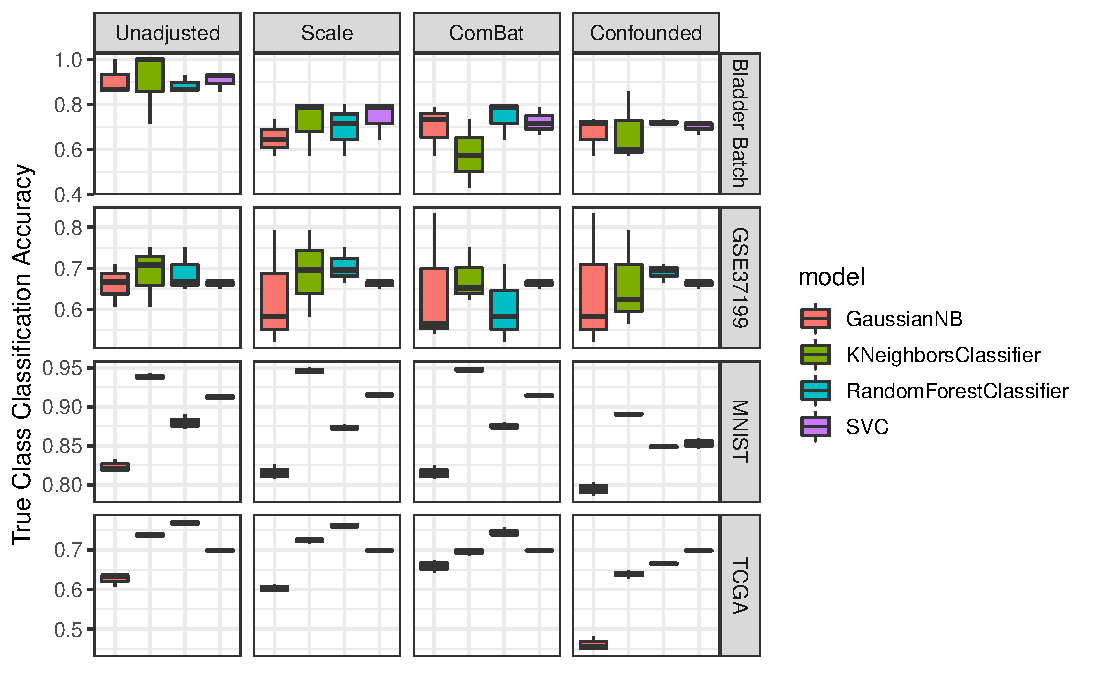
\includegraphics[width=\columnwidth]{figures/final/true_class_accuracy.pdf}
	\caption[True class classification accuracy]{\textbf{True class classification accuracy} for several datasets and adjusters with 4-fold cross-validation repeated 3 times. A higher accuracy after adjustment is desired because it represents that the adjuster has not destroyed the true class signal.
	See also Table \ref{tab:true_class}.}
	\label{fig:true_class}
\end{figure}
\begin{table}
	\centering
	\centering\rowcolors{2}{gray!6}{white}

\begin{tabular}{l|l|r|r|r|r|r}
\hiderowcolors
\hline
Dataset & Adjustment & Baseline & GaussianNB & KNeighbors & RandomForest & SVC\\
\hline
\showrowcolors
 & Unadjusted &  & 0.9079365 & 0.9047619 & 0.8841270 & 0.9063492\\
\cline{2-2}
\cline{4-7}
 & Scale &  & 0.6492063 & 0.7190476 & 0.6952381 & 0.7428571\\
\cline{2-2}
\cline{4-7}
 & ComBat &  & 0.6968254 & 0.5777778 & 0.7428571 & 0.7222222\\
\cline{2-2}
\cline{4-7}
\multirow[t]{-4}{*}{\raggedright\arraybackslash Bladder Batch} & Confounded & \multirow[t]{-4}{*}{\raggedleft\arraybackslash 0.7017544} & 0.6730159 & 0.6761905 & 0.7206349 & 0.6984127\\
\cline{1-7}
 & Unadjusted &  & 0.6612319 & 0.6890097 & 0.6896135 & 0.6618357\\
\cline{2-2}
\cline{4-7}
 & Scale &  & 0.6322464 & 0.6902174 & 0.7041063 & 0.6618357\\
\cline{2-2}
\cline{4-7}
 & ComBat &  & 0.6467391 & 0.6757246 & 0.6044686 & 0.6618357\\
\cline{2-2}
\cline{4-7}
\multirow[t]{-4}{*}{\raggedright\arraybackslash GSE37199} & Confounded & \multirow[t]{-4}{*}{\raggedleft\arraybackslash 0.6666667} & 0.6461353 & 0.6606280 & 0.6902174 & 0.6618357\\
\cline{1-7}
 & Unadjusted &  & 0.8236658 & 0.9388265 & 0.8801867 & 0.9128345\\
\cline{2-2}
\cline{4-7}
 & Scale &  & 0.8160683 & 0.9462902 & 0.8743188 & 0.9153669\\
\cline{2-2}
\cline{4-7}
 & ComBat &  & 0.8152686 & 0.9478891 & 0.8755154 & 0.9140346\\
\cline{2-2}
\cline{4-7}
\multirow[t]{-4}{*}{\raggedright\arraybackslash MNIST} & Confounded & \multirow[t]{-4}{*}{\raggedleft\arraybackslash 0.1135000} & 0.7944837 & 0.8907100 & 0.8484595 & 0.8528601\\
\cline{1-7}
 & Unadjusted &  & 0.6251933 & 0.7380770 & 0.7675432 & 0.6979360\\
\cline{2-2}
\cline{4-7}
 & Scale &  & 0.6028491 & 0.7232736 & 0.7602833 & 0.6979360\\
\cline{2-2}
\cline{4-7}
 & ComBat &  & 0.6590746 & 0.6953731 & 0.7444855 & 0.6979360\\
\cline{2-2}
\cline{4-7}
\multirow[t]{-4}{*}{\raggedright\arraybackslash TCGA} & Confounded & \multirow[t]{-4}{*}{\raggedleft\arraybackslash 0.6979500} & 0.4612043 & 0.6387186 & 0.6651957 & 0.6979360\\
\hline
\end{tabular}
\rowcolors{2}{white}{white}
	\caption[True class classification accuracy]{
		\pdfbookmark[1]{Table \ref{tab:true_class}}{true_class}
		\textbf{True class classification accuracy} for several datasets and adjusters.
		After adjustment by the ideal batch adjuster, all true class signal should be preserved, and all classifiers should therefore have the same accuracy in predicting true class before and after adjustment.
		See also Figure \ref{fig:true_class}.
	}
	\label{tab:true_class}
\end{table}

\begin{figure}
	\pdfbookmark[1]{Figure \ref{fig:mnist}}{asdf}
	\centering
	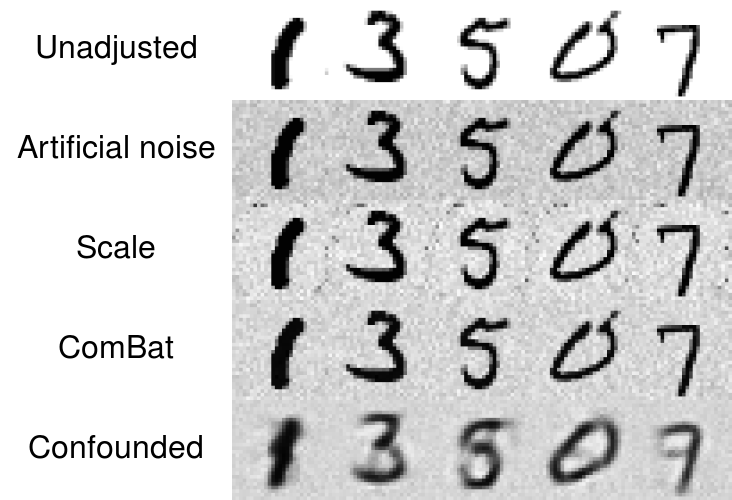
\includegraphics[width=\columnwidth]{figures/final/mnist.png}
	\caption[MNIST handwritten digits]{\textbf{MNIST handwritten digits}
	\begin{enumerate*}[(a)]
		\item before any adjustment,
		\item with artificial noise added,
		\item adjusted for noise by the scale adjuster,
		\item adjusted for noise by ComBat, and
		\item adjusted for noise by Confounded.
	\end{enumerate*}
	Although Confounded seems to remove more noise from the background, it struggles in some cases to accurately replicate the input data.}
	\label{fig:mnist}
\end{figure}

\section{Discussion} \label{sec:discussion}

\textbf{Why should I use a neural network for batch adjustment?}
The process of measuring data typically leaves confounding effects, especially when the data or measurement process involves living things.
Imagine an experiment where two researchers measure the length of caterpillars.
If one researcher is left-eye dominant and the other is right-eye dominant, they may each see lengths as being a millimeter different.
If both researchers use the same wooden ruler at different relative humidities, the measurements may come out differently due to the wood swelling or due to the caterpillars reactions to humidity.
These same types of problems exist when measuring expression levels, but to more of an extreme---in addition to the target values and measuring equipment changing slightly due to systemic factors, the target values also change in response to each other.
Each of the 20,000 transcript levels may influence or be influenced by other transcript levels.
These cascading network-like effects are extremely likely to have nonlinear components, and our research shows that these nonlinear effects do indeed exist in gene expression data, thus rendering linear batch correction methods insufficient.
Therefore, some form of nonlinear adjustment must be used in order to correct for real-world confounding effects.
Rather than individually model each of infinitely many possible nonlinear interactions to see which represent confounders, we can use a neural network to both approximate and remove the confounders, since neural networks are proven to be universal function approximators \citep{csaji_approximation_2001}.

\textbf{How can I tell how well batch adjustment worked?}
Although the metrics and figures that have been used in the past to validate batch adjustment (such as PCA, MSE, and MMD) represent how well linear effects have been removed, they cannot completely display whether two batches are distinguishable from one another.
Machine learning algorithms are designed specifically to tease out patterns in data that may distinguish one group from another.
We suggest to users of batch correction software that they use machine learning classification accuracy before and after correction in order to determine the degree of batch removal.
We also suggest to researchers in the field of batch correction that classification accuracy be used as a metric in validating their software.
Specifically, the Random Forests algorithm \citep{tin_kam_ho_random_1995} seems to work very well and runs relatively quickly on gene expression data.

\textbf{Which batch adjuster should I use?}
In our testing, ComBat did very well with small ($n < 100$) datasets, even with removing any identifiable nonlinear effects.
However, Confounded outperformed ComBat on the larger datasets according to the batch classification accuracy metric.
In addition to dataset size, researchers selecting a batch adjustment algorithm should consider how important it is for them to accurately replicate their input data.
Such researchers can adjust Confounded's $\lambda$ parameter in order to balance the tradeoff of removing batch and matching the inputs.

\textbf{What limitations does Confounded have?}
\begin{enumerate*}[(a)]
	\item Confounded uses a variational autoencoder, which are known for often outputting a blurry version of the input data (as can be seen in Figure \ref{fig:mnist}).
	However, recent work has identified modifications that may be made to the basic VAE structure to make output images sharper and more realistic \citep{hou_deep_2016}.
	Similar research with variational autoencoders and gene expression data may yield improved reconstruction losses and decrease the blurring effect.
	\item Confounded takes a long time to run in comparison with ComBat and other linear adjusters.
	Although we acknowledge this as a downfall of many types of machine learning and of neural network in particular, we believe that 30-60 minutes is a reasonable amount of time for a step that will be run only once per pipeline and that can greatly improve data quality.
	\item It can be difficult to identify the optimal network structure and parameter set for a neural network.
	Though this is the case for many applications of neural networks, we feel that Confounded's default structure worked well in our testing and that it will suffice for most batch correction applications.
	\item Neural networks usually perform better when given large amounts of data, and traditional batch datasets typically have very few samples.
	We did find that ComBat may outperform Confounded on many smaller, more traditional datasets, but that Confounded performs better on larger datasets.
	However, Confounded did perform reasonably well with the smaller datasets and appeared to avoid overfitting.
	In cases where ComBat is unable to completely remove confounding effects in a small dataset, Confounded may be a viable replacement method.
\end{enumerate*}

\textbf{What else might Confounded be used for?}
At its root, batch correction is a data integration problem:
data from multiple batches must have batch-specific confounding effects removed in order to be treated as one dataset.
Confounded shows promise in removing traditional batch effects from microarray expression data in the Bladderbatch and GSE37199 datasets.
It also effectively decreased artificial batch effects in image data and cancer-type-specific confounding effects in RNA-Seq data.
Confounded may be effective in other data integration problems, such as combining microarray with RNA-Seq datasets, or merging several large datasets measured under different conditions.

Confounded, and adversarial autoencoders in general, show promise as a valuable way to remove confounding biases from expression datasets.
Such methods will enable researchers access to larger datasets, therefore increasing the scope of analyses and furthering science as a whole.

\newpage
\phantomsection
\addcontentsline{toc}{section}{References}
\bibliography{references}

\end{document}
